\section{Structural Subsystem \label{structural}}

\subsection{Manufacturing and layout}
The finalised structure is represented in the computer render of figure \ref{ExplodedSat}. The external structure consists of 6061-T6 (space grade) Aluminium that has been CNC machined to within 0.1 mm maximum tolerance. Material properties for this structure are shown in table \ref{Materials}. The design itself is based on the ISIS structure, a flight proven commercial structure that has been quality tested for vibration, vacuum cycling, thermal cycling and stress. Assembly involves joining four ribs to two side frames using M3 bolted connections through countersunk un-threaded holes. Commercial GaAs solar panels and aluminium plates form the remainder of the external enclosure. \\
  
\begin{figure}[!h]
\centering	
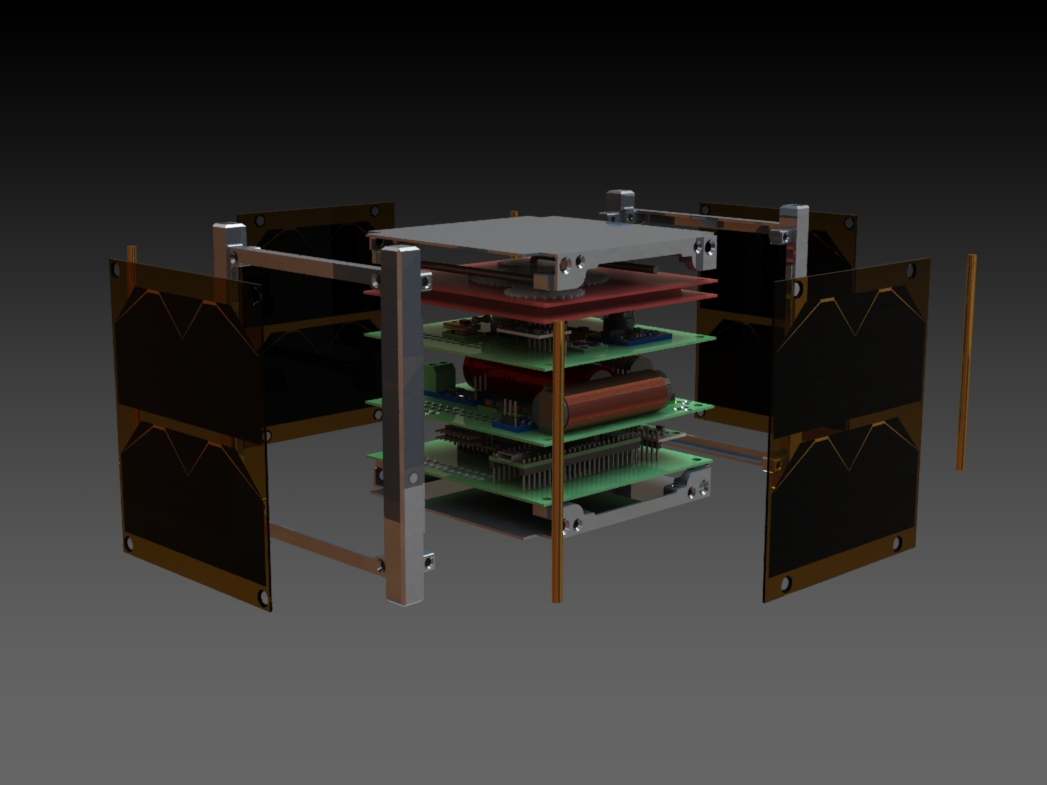
\includegraphics[width=\textwidth]{ExplodedSat.JPG}
\caption{External exploded view of the MuirKat's final layout}
\label{ExplodedSat}
\end{figure}

The internal structure is custom to the MuirKat. The lower PCB contains the OBC and communications subsystems primary components, the middle PCB contains the ADCS and EPS subsystem, and the top two structures contain the payload PCB and deployment structure respectively. The PCBs themselves are glass fibre reinforced epoxy composites (FR4) with material properties as per those of table \ref{Materials}. The payload structure was manufactured using 3D printed (fused deposition modelling) ABS. The Langmuir probes are 2mm cold drawn stainless steel. \\ 

The assembly mechanism to connect the internal and external structures together involves steel spacers. These thread into each other, locking all the PCBs in place, then thread to the MuirKat structure itself. In organising the layout, heavier components were kept central in order to keep the centre of mass within the required 20 mm sphere (measured from geometric centre). Using SolidWorks the centre of mass is calculated as shown in table \ref{COM}. The value calculated is at most 6.89mm away from the geometric centre (50,50,50). In addition, the entire assembly conforms to the required directional launch standards as all PCBs align with the negative Z direction. 
  
\begin{table}[H]
\centering
\begin{tabular}{@{}lcccl@{}}
\toprule
                        & \textbf{6061-T6 Aluminium} & \textbf{FR4} & \textbf{ABS} & \textbf{Stainless Steel} \\ \midrule
  Young's Modulus (GPa) & 68.9                       & 21           & 2.5          & 193                      \\
  Density (kg/m$^{3}$)  & 2700                       & 1850         & 850          & 7700                     \\
 Poisson's Ratio       & 0.33                       & 0.118        & 0.35         & 0.30                     \\
 Yield Strength (MPa)  & 310                        & 70           & 40           & 215                      \\ \bottomrule
\end{tabular}
\caption{Material properties of core structural materials}
\label{Materials}
\end{table}
 
\begin{table}[]
\centering
\begin{tabular}{@{}lll@{}}
\toprule
\textbf{X (mm)} & \textbf{Y (mm)} & \textbf{Z (mm)} \\ \midrule
 49.89           & -46.98          & 56.11           \\ \bottomrule
\end{tabular}
\caption{Centre of Mass with frame of reference as illustrated in figure \ref{fig:COM}. The MuirKat satisfies QB50 requirements, keeping the COM within a 20 mm sphere from geometric centre}
\label{COM}
\end{table}
 
\begin{figure}
\centering	
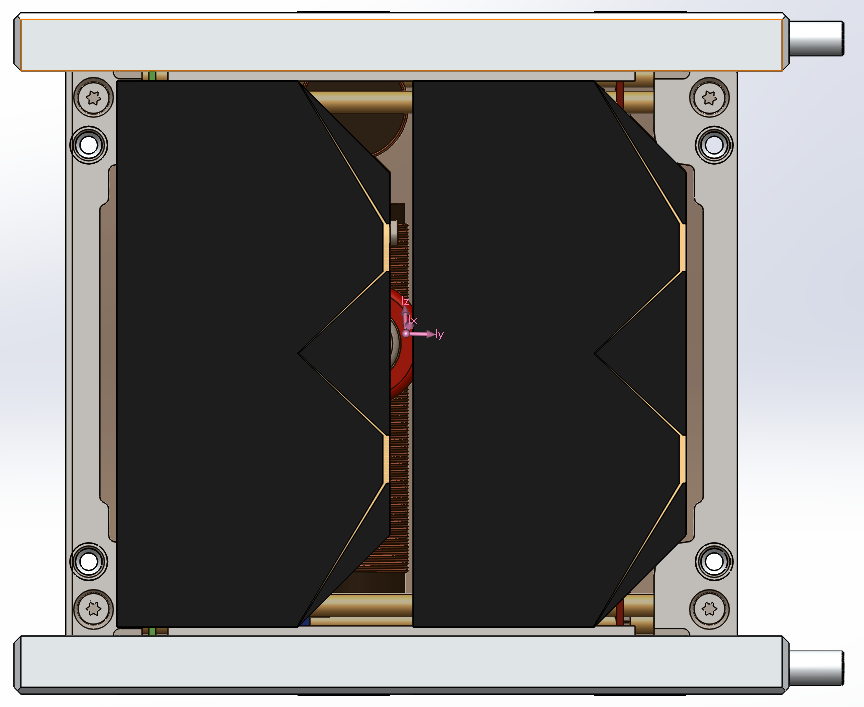
\includegraphics[width=0.65\textwidth]{COM.PNG}
\caption{Centre of mass represented by the pink axes, reference coordinate system placed at the base of the side frame's top right corner}
\label{fig:COM}
\end{figure}
  
\begin{figure}
\centering	
\includegraphics[width=\textwidth]{coordinates}
\caption{Coordinate axes demonstrating - Z alignment of the MuirKat}
\end{figure}

\subsection{Mass Budget}
A detailed mass budget is attached in the appendix, a summary is represented here in table \ref{StrucBudget}. Approximately 60\% of the available mass was utilised. One might consider this under-design, however since the MuirKat successfully meets all the mission requirements as well as the QB50 mass requirements this is not a cause for concern. 
\begin{table}[!h]
\centering
\begin{tabular}{@{}lccc@{}}
\toprule
\textbf{}          & \textbf{}                     & \multicolumn{2}{c}{\textbf{Mass}}      \\ \midrule
\textbf{Subsystem} & \textbf{Number of Components} & \textbf{Mass}   & \textbf{Contingency} \\
OBC                & 12                            & 107.50          & 10.75                \\
EPS                & 6                             & 47.70           & 2.12                 \\
TTC                & 12                            & 29.40           & 2.51                 \\
Payload            & 17                            & 18.14           & 4.60                 \\
ADCS               & 22                            & 143.51          & 37.00                \\
Structure          & 9                             & 213.21          & 21.00                \\
Thermal            & 1                             & 50.00           & 0.10                 \\
\textbf{Total}     & \textbf{79}                   & \textbf{609.46} & \textbf{687.54}      \\ \bottomrule
\end{tabular}
\caption{Summary Mass Budget}
\label{StrucBudget}
\end{table}

\subsection{Simulation Method}
To perform finite element analysis a simulation criterion is required. All simulations consider a typical CubeSat launch such as those from a P-Pod launcher or NanoRack system. This involve keeping the negative Z face fixed, but allowing the positive Z face to have a small displacement. This displacement arises due to the kill switch not being rigidly fixed when in contact with the launch armature. The frame itself is also not a rigid structure, relying on M3 bolts to join all elements. To simulate this, all contacts between the frames and ribs were suppressed. A typical P-Pod launch structure is shown in figure \ref{fig:P-Pod}. 
  
 \begin{figure}[H]
 \centering	
 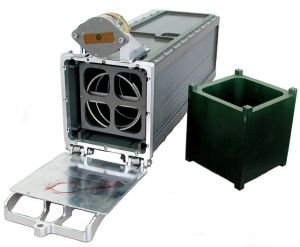
\includegraphics[width=0.5\textwidth]{P-Pod.jpg}
 \caption{Illustration of a typical P-Pod launch system for CubeSat deployment. Available at \text{http://www.pe0sat.vgnet.nl/wp-content/uploads/2011/11/P-Pod-Launcher.jpg} [Accessed October 29 2017]}
 \label{fig:P-Pod}
 \end{figure}
 
% Modes 
\subsection{Modal Analysis}
The modal analysis produced interesting results, highlighting the structural weakness that is the Langmuir probe. The first 5 modes at three mesh sizes are shown in table \ref{table:modes}. The solution appears to begin to converge for lower modes (expected 240-245 Hz convergence point), however the higher modes still demonstrate a level of uncertainty. Unfortunately the finest mesh (3 mm) was the computing limit of the hardware available for this project and so we settle for the results in table \ref{table:modes}. \\

\begin{table}[]
\centering
\begin{tabular}{@{}lccccc@{}}
\toprule
\multicolumn{1}{c}{\textbf{Element Size (mm)}} & \textbf{Mode 1 (Hz)} & \textbf{Mode 2 (Hz)} & \textbf{Mode 3 (Hz)} & \textbf{Mode 4 (Hz)} & \textbf{Mode 5 (Hz)} \\ \midrule
10                                             & 253.34               & 254.41               & 255.72               & 258.42               & 393.64               \\
5                                              & 253.29               & 253.73               & 254.43               & 257.41               & 350.75               \\
3                                              & 247.03               & 249.11               & 249.32               & 250.49               & 354.98               \\ \bottomrule
\end{tabular}\caption{Results of Modal Analysis}
\label{table:modes}
\end{table} 

The first 4 modes provide the most interesting discussion due to their close spacing. Observing figure \ref{fig:mode1} we account for this by reasoning the Langmuir probes acts as an elastic beam. Keeping the probes free at one end means they have poor vibration performance, noticeable by observing how the 5th mode (the first due to the structure alone, as shown in figure \ref{fig:mode5}) is approximately 100 Hz away from the first mode due to the langmuir probes. If the probes were to be fixed we would expect to achieve a 100 Hz improvement in vibration performance. However, this we would lose all the benefits of the spur gear payload mechanism and instead return to what was expected of a torsion spring system. As such the decision to keep the payload structure as it stands was preferred, primarily due to the fact that the fundamental mode is still well above the 90 Hz requirement (QB50). 

\begin{figure}[H]
\centering	
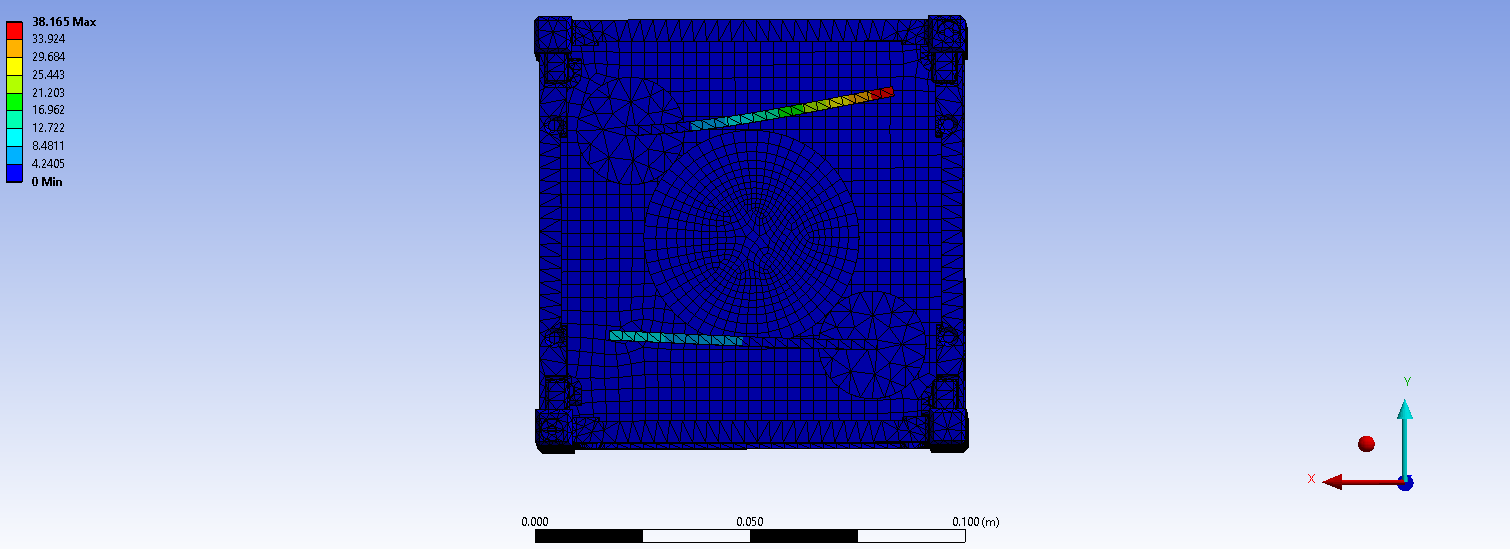
\includegraphics[width=\textwidth]{mode1}
\caption{Simulation result of the first mode at finest mesh (247.03 Hz). The Langmuir probes acts as elastic beams and prove a considerable weakpoint within the structure. Scale in units 1e-3 meters, i.e max deflection 3.8 mm}
\label{fig:mode1}
\end{figure}

\begin{figure}[H]
\centering	
\includegraphics[width=\textwidth]{mode5}
\caption{Simulation result for the fifth mode at finest mesh (354.98 Hz). This is the first mode due to the structure as a whole instead of the Langmuir probes}
\label{fig:mode5}
\end{figure}


% Acceleration 
\subsection{Quasistatic Acceleration Analysis}

With the simulation method remained unchanged a constant acceleration load of 10.8g was applied along each coordinate axes as per QB50 requirements. The results for the three cases are summarised in table \ref{table:stresses}. \\ 

\begin{table}[]
\centering
\begin{tabular}{@{}lccc@{}}
\toprule
\textbf{Element Size (mm)} & \multicolumn{1}{l}{\textbf{Max Stress X (MPa)}} & \multicolumn{1}{l}{\textbf{Max Stress Y (MPa)}} & \multicolumn{1}{l}{\textbf{Max Stress Z (MPa)}} \\ \midrule
10                         & 20.6                                            & 32.8                                            & 7.3                                             \\
5                          & 23.8                                            & 33.5                                            & 7.6                                             \\
3                          & 24.2                                           & 34.1                                             & 7.6                                             \\ \bottomrule
\end{tabular}
\caption{Maximum stress values calculated using FEA under 10.8g acceleration load}
\label{table:stresses}
\end{table}

The maximum stress listed uses the Von-Mises energy method of calculation. This is considered the best indication of yielding behaviour. Using table \ref{Materials} we see that no component will experience a stress larger than it's yield value. The weakest structural element is the ABS plastic used in the payload at 40 MPa. The largest maximum stress occurs along the Y direction, appearing to converge at 35 MPa. This indicates a factor of safety of 1.15, a relatively tight tolerance. If the satellite was given a longer development cycle the payload would be re-made using better materials (preferably the same FR4 composite for the base and aluminium for the gears), this would raise the factor of safety to 1.75. \\

In addition to these stress values, the total deformation of the structure is a useful visualisation tool. Figures \ref{fig:defX}, \ref{fig:defX} and \ref{fig:defX} explicitly demonstrate how the cubesat deforms inside the P-Pod. All values are on the order $1\times 10^{-5} \ \text{m}$ and the MuirKat is considered space-ready from a structural standpoint. 

\begin{figure}[H]
\centering	
\includegraphics[width=\textwidth]{deformationX}
\caption{Total deformation of the MuirKat in the X direction. Along the X axis the deformation is distributed primarily throughout the internal structure, as supported by the equivalent stress value that lies between the maximum and minimum values seen along all axis.}
\label{fig:defX}
\end{figure}

\begin{figure}[H]
\centering	
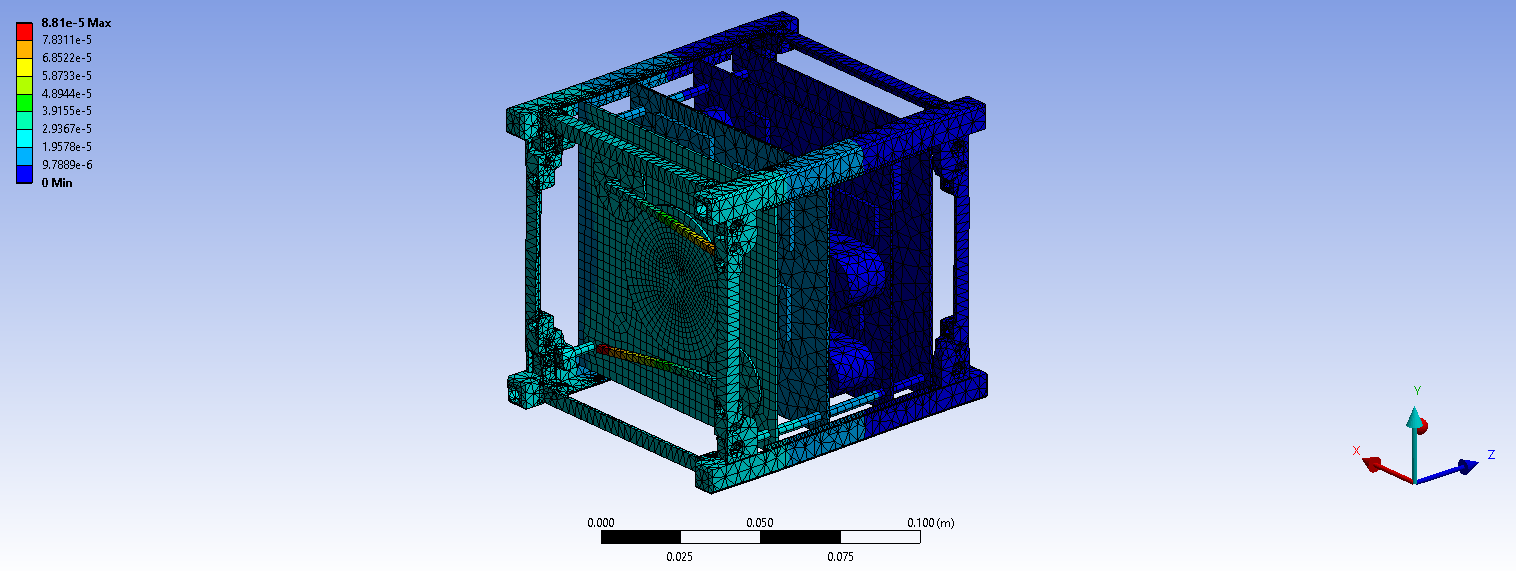
\includegraphics[width=\textwidth]{deformationY}
\caption{Total deformation of the MuirKat in the Y direction. The Y direction contained the highest stress and deformation figures, this is due to the fact they the acceleration occurs in the same direction as the resonant deflection of the Langmuir probes. Again, leaving these probes free proved to be a considerable weak point within the structure.}
\label{fig:defY}
\end{figure}

\begin{figure}[H]
\centering	
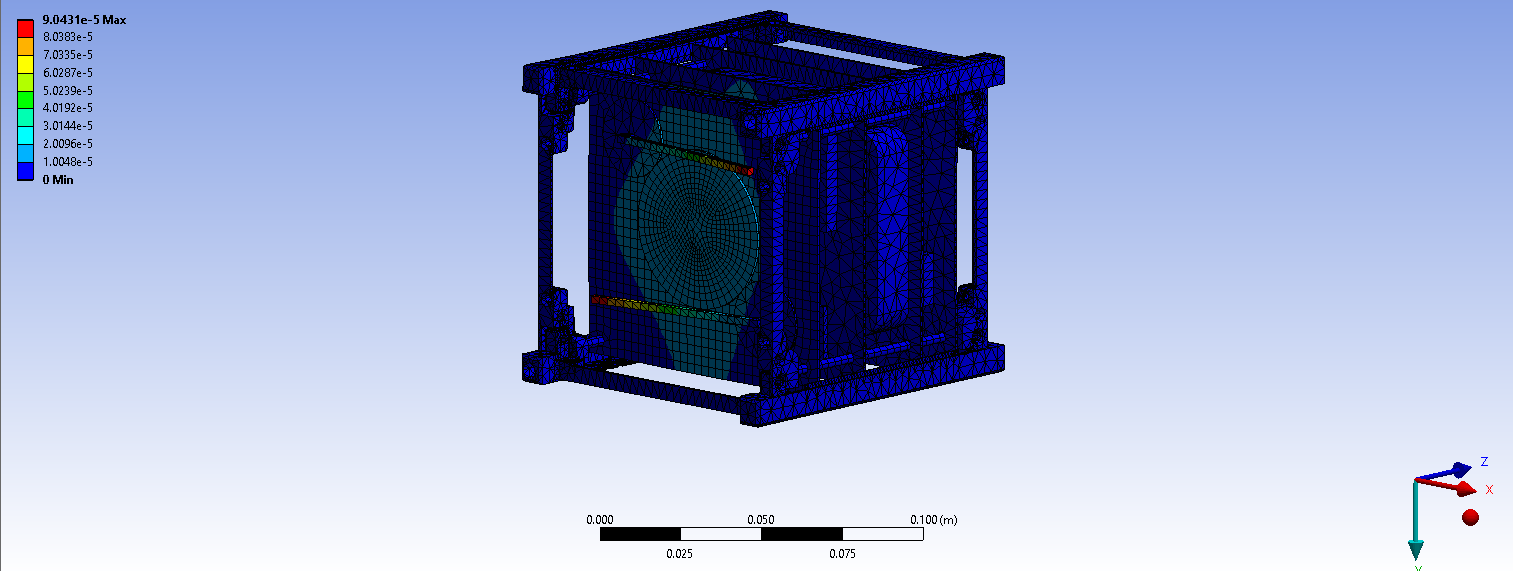
\includegraphics[width=\textwidth]{deformationZ}
\caption{Total deformation of the MuirKat in the Z direction. This axis did not see large values of stress or deformation, attributed to the fact that both Aluminium and FR4 are strong in compression. Noticeably the ABS plastic (and of course the probes) are the weak elements in this coordinate direciton.}
\label{fig:defZ}
\end{figure}
